
\documentclass[a4paper,12pt]{article}

\usepackage{ucs}
\usepackage[utf8x]{inputenc}
%\usepackage[latin1]{inputenc}
\usepackage[T1]{fontenc}

\usepackage[french]{babel}

\pagestyle{plain}

\usepackage{graphicx}
\usepackage{subfigure}
\DeclareGraphicsExtensions{.pdf,.eps,.jpg,.png,.gif}

\usepackage{color}
\definecolor{grey}{rgb}{0.9,0.9,0.9}
\definecolor{teal}{rgb}{0.0,0.5,0.5}
\definecolor{violet}{rgb}{0.5,0,0.5}

\usepackage{listings}
\usepackage{listingsutf8}
\lstloadlanguages{[Visual]C++}
\lstdefinestyle{listing}{
  language=Java,
  captionpos=t,
  inputencoding=utf8/latin1,
  extendedchars=true,
  resetmargins=true,
  xleftmargin=-60pt,
  xrightmargin=-70pt,
%  frame=single,
  numbers=left,
  numberstyle=\tiny,
  numbersep=5pt,
  breaklines=true,
  breakatwhitespace=true,
  showspaces=false,
  showstringspaces=false,
  showtabs=false,
  tabsize=2,
  basicstyle=\footnotesize\ttfamily,
  backgroundcolor=\color{grey},
  keywordstyle=\color{blue}\bfseries,
  commentstyle=\color{teal},
  identifierstyle=\color{black},
  stringstyle=\color{red},
  numberstyle=\color{violet},
}
\lstset{style=listing}

%%%%%%%%%%%%%%%%%%%%%%%%%%%%%%%%%%%%%%%%%%%%%%%%%%%%%%%%%%%%

\author{
  Quentin \textsc{Augrain}, Florent \textsc{Mallard} \\ \\
  INSA de Rennes \\
  5INFO
}

\title{Projet de Modélisation et Ingénierie du vivant}

\begin{document}
\maketitle

\section{Tutoriel}

Question 1: Comme indiqué dans les commentaires de la fonction, il y a deux fonctions dans la boucle :
\begin{itemize}
    \item Bouger le monde;
    \item Afficher le monde.
\end{itemize}

Cela signifie que la fonction va tout d'abord calculer le prochain mouvement, pour ensuite afficher la nouvelle position. Pour le moment, la phase de calcul n'est pas implémentée et rien ne bouge dans la simulation.

Question 2: Nous ajoutons la gravité au \og{}force_accumulator\fg{}, et obtenons le résultat montré à la \textsc{Figure} \ref{fig:q2}, c'est-à-dire que rien ne se passe. En effet même si nous calculons maintenant les forces, nous ne les appliquons pas au mesh, ce qui résulte en un mesh toujours fixe. Il nous faut donc appliquer ces forces à chaque particule du mesh afin qu'un effet se fasse ressentir.
\begin{figure}
  \centering
  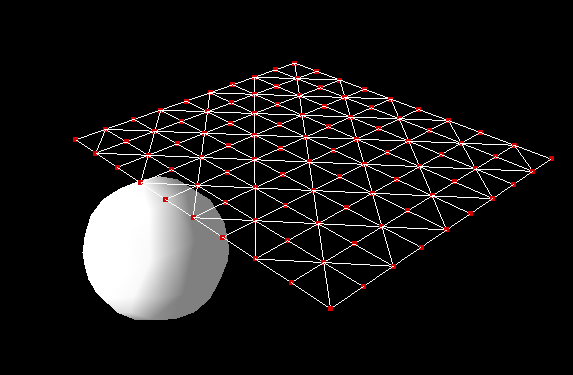
\includegraphics{q2.png}
  \caption{Aucun changement n'est visible même si les forces changent.}
  \label{fig:q2}
\end{figure}

Question 3: Maintenant que nous appliquons les forces, le mesh tombe et finit par disparaître de l'écran. Il semble qu'il n'y ait pas de limite physique à sa chute. On peut donc envisager un moyen afin que même si aucune autre interaction que la gravité ne s'applique au mesh, il reste dans le champ de l'écran.

Question 4 : Une autre solution a été proposée, il s'agit de fixer le premier rang des particules. Ainsi, le mesh reste visible et a un effet dit \og{}de rideau\fg{}. Pour ce faire, il nous faut nullifier les forces de ces particules. Nous avons compté dix particules sur ce rang, nous avons donc ajouté une boucle comme montré sur la \textsc{Figure} \ref{fig:q4}. Cette boucle met simplement les forces appliquées à ces dix particules à zéro, empêchant ainsi tout mouvement.
\begin{figure}
  \centering
  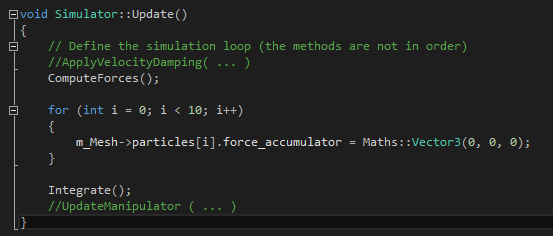
\includegraphics{q4.png}
  \caption{Le premier rang reste fixe.}
  \label{fig:q4}
\end{figure}

Question 5 : Le comportement est pour le moins étrange, car les particules oscillent de plus en plus jusqu'à disparaître. Pour le moment la simulation n'est pas stable, car les forces appliquées aux particules ne se compensent pas. Ceci aboutit, plus ou moins rapidement en fonction des paramètres de simulation choisis, à un écran contenant uniquement le premier rang de particules, demeuré fixe comme précisé à la question précédente.
La \textsc{Figure} \ref{fig:q5} montre notre implémentation.
\begin{figure}
  \centering
  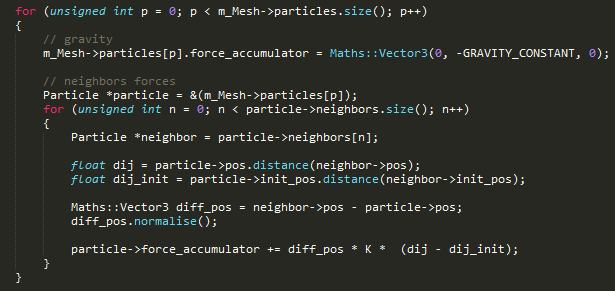
\includegraphics{q5.png}
  \caption{Mise à jour des voisins pour chaque particule.}
  \label{fig:q5}
\end{figure}

Question 6 : Le paramètre \og{}dt\fg{} définit la vitesse de la simulation à travers le nombre d'itérations à chaque fois. Une valeur plus petite correspond donc à une simulation plus rapide, car on calcule la position et les forces après un instant plus grand, le mouvement a donc été plus important.
K définit la rigidité. Celle-ci va aider à obtenir l'effet de rideau désiré. Sachant cela, nous n'avons pas réussi à stabiliser la simulation. En effet même si le rideau est considéré comme plus rigide, les forces des particules ne se compensent pas et donnent le même résultat que précédemment.

Question 7 : Nous ajoutons la boucle demandée qui effectue \textit{n} appels à \og{}Update\fg{} avec un timestep désormais divisé par \textit{n}. Le but de cette manipulation est d'avoir un mouvement plus petit, car calculé sur un plus petit pas de temps. Grâce à cela les interactions calculées sont plus fines et donc plus réalistes. Bien entendu, cela implique aussi plus de calculs, et donc un coût plus important pour le processeur. Le CPU est bien plus actif après que nous ayons implémenté cette modification. 

Question 8 : En amortissant la chute des particules, nous arrivons à stabiliser la simulation. L'amortissement simule l'interaction des particules avec l'air ambiant. C'est lui qui va réussir à compenser les interactions des particules entre elles et empêcher une oscillation de plus en plus importante comme observée précédemment. 
%TODO Image(s) de la chute et/ou du résultat
%\begin{figure}
%  \centering
%  \includegraphics{}
%  \caption{Le mesh ressemble à un rideau pendant.}
%  \label{fig:}
%\end{figure}

Question 9 : 	Avec dt = 1/200, K = 300, et n = 20, nous arrivons à une simulation stable. Mais ces paramètres sont très coûteux en ressources car avec dt = 1 / 200 et n = 20, cela signifie que nous effectuons quatre mille fois la boucle \og{}Update\fg{} par seconde. Plus tard, et sur des ordinateurs moins puissants, nous préférerons utiliser un dt de 1/50. Cela n'affecte pas trop la simulation mais permet de diminuer significativement le coût en ressources.

Question 10 : Le modèle de Mass-Spring-Damper est assez simple à utiliser dès lors que les formules à appliquer sont à disposition. En revanche, pour obtenir une simulation stable, le moindre écart dans les paramètres peut créer une simulation tout à fait exotique. En effet nous avons vu que diminuer la rigidité du mesh pouvait conduire à une simulation qui n'était pas réaliste, car le mesh se comportait plus comme une plaque pivotante que comme un rideau. Appliquer un amortissement trop fort rend la simulation trop longue pour être réaliste.

\section{TP2}

Question 1 : Baisser la valeur d'amortissement résulte en une accélération de la chute et en une baisse de la stabilité. En effet, l'amortissement sert à compenser les interactions entre les particules, qui font osciller le mesh, et à simuler une interaction avec l'air. Diminuer ces \og{}frottements\fg{} accèlère donc la chute du rideau, et les particules ont des interactions plus fortes qui déstabilisent la simulation. Après quelques recherches, la vitesse relative est simplement une soustraction des vecteurs vitesses du voisin par rapport à la particule.

Question 2 : Afin de simuler le sol, nous implémentons une limite de hauteur en dessous de laquelle les particules ne peuvent descendre, ayant pour effet de simuler un plan. Cette méthode nous a posé un petit problème lorsque 
%TODO image sol + code
%\begin{figure}
%  \centering
%  \includegraphics{}
%  \caption{Implémentation du sol.}
%  \label{fig:}
%\end{figure}

%\begin{figure}
%  \centering
%  \includegraphics{}
%  \caption{Rideau tombé sur le sol.}
%  \label{fig:}
%\end{figure}

Question 3 : Nous avons simplement changé la couleur de notre manipulator, que nous montrons ci-dessous : %TODO
%\begin{figure}
%  \centering
%  \includegraphics{}
%  \caption{Le manipulateur est maintenant de couleur rouge.}
%  \label{fig:}
%\end{figure}


Question 4 : Le coefficient C, s'il est négatif, créé une attraction entre le manipulator et le mesh. En revanche, s'il est positif, les deux objets se repoussent.

Question 5 : %TODO code
%\begin{figure}
%  \centering
%  \includegraphics{q5_tp2.png}
%  \caption{Ajout du client haptique.}
%  \label{fig:q5tp2}
%\end{figure}

Question 6 :%TODO code
%\begin{figure}
%  \centering
%  \includegraphics{}
%  \caption{Ajout de la force en retour.}
%  \label{fig:}
%\end{figure}

Question 7 :%TODO code
%\begin{figure}
%  \centering
%  \includegraphics{}
%  \caption{Ajout du clic avec le client haptique.}
%  \label{fig:}
%\end{figure}

Question 8 :%TODO code
%\begin{figure}
%  \centering
%  \includegraphics{}
%  \caption{Le mesh ressemble à un rideau pendant.}
%  \label{fig:}
%\end{figure}

Question 9 :%TODO scrshot
%\begin{figure}
%  \centering
%  \includegraphics{}
%  \caption{Mesh représentant un foie.}
%  \label{fig:}
%\end{figure}

Question 10 :%TODO scrshot avec les positions des sphères
%\begin{figure}
%  \centering
%  \includegraphics{}
%  \caption{Le mesh du foie fixé.}
%  \label{fig:}
%\end{figure}

%\begin{figure}
%  \centering
%  \includegraphics{}
%  \caption{Implémentation de la fixation des points.}
%  \label{fig:}
%\end{figure}

Question 11 : Afin d'atteindre les objectifs fixés, nous avons fixé une dizaine de points, un time step de 1/50e de seconde, et 20 boucles avant d'afficher le résultat.

\section{TP3}

Question 1 :

Question 2 : Afin de mieux repérer les particules fixées, nous avons décidé de les colorer en bleu.
% Image points fixés
%\begin{figure}
%  \centering
%  \includegraphics{}
%  \caption{Le mesh resemble à un rideau pendant.}
%  \label{fig:}
%\end{figure}

Question 3 : Nous avons choisi de fixer des points à l'intérieur du foie, afin que la simulation soit plus réaliste. En effet, de cette manière nous préservons la \og{}texture\fg{} du foie en autorisant la partie supérieure à bouger, comme si le foie était posé. Nous avons également souhaité conserver les lobes du fois afin de pouvoir les soulever.

Question 4 : Nous avons choisi de sauvegarder les particules fixées dans un fichier de type texte, nommé \og{}save\fg{}. Si ce fichier existe déjà, il est chargé au lancement du programme. Celui-ci est écrasé à chaque appui sur la touche \og{}s\fg{}, ne laissant la possibilité que d'avoir une seule sauvegarde, à moins de la renommer manuellement.
%\begin{figure}
%  \centering
%  \includegraphics{}
%  \caption{Le mesh resemble à un rideau pendant.}
%  \label{fig:}
%\end{figure}

Question 5 : Afin de permettre l'usage de la souris et du moniteur haptique au cours de la même simulation, nous avons ajouté une variable \og{}mode\fg{}, changée par l'appui sur la touche \og{}m\fg{}, qui permet d'autoriser le changement de position avec le moniteur haptique.
% Image de code
%\begin{figure}
%  \centering
%  \includegraphics{}
%  \caption{Le mesh resemble à un rideau pendant.}
%  \label{fig:}
%\end{figure}

Question 6 : Afin d'avoir un contrôle plus précis, nous avons implémenté un facteur permettant d'amplifier ou de diminuer les mouvements du manipulateur. Celui-ci est contrôlé par \og{}+\fg{} et \og{}-\fg{} pour augmenter ou diminuer sa valeur, par seuil de 0.2.
%code
%\begin{figure}
%  \centering
%  \includegraphics{}
%  \caption{Le mesh resemble à un rideau pendant.}
%  \label{fig:}
%\end{figure}

Question 7 : Voici la manière dont nous avons choisi d'implémenter une forme d'inertie à notre manipulateur lorsque le bras articulé arrive en bout de course :
%code
%\begin{figure}
%  \centering
%  \includegraphics{}
%  \caption{Le mesh resemble à un rideau pendant.}
%  \label{fig:}
%\end{figure}
% Image manipulateur loin
%\begin{figure}
%  \centering
%  \includegraphics{}
%  \caption{Le mesh resemble à un rideau pendant.}
%  \label{fig:}
%\end{figure}

Question 8 : Nous avons choisi d'appuyer sur un des boutons du bras articulé afin de désactiver le mouvement du manipulateur. De cette manière nous pouvons remettre le bras à la position désirée avant de reprendre la manipulation.
%code
%\begin{figure}
%  \centering
%  \includegraphics{}
%  \caption{Le mesh resemble à un rideau pendant.}
%  \label{fig:}
%\end{figure}
\end{document}
